\subsection{Risoluzione di Sistemi di Equazioni Lineari}

\subsubsection{Metodi diretti}

Si consideri la matrice di dimensione $n \times n$:
\begin{equation*}
    A = \begin{bmatrix}
        1 & 1 & 1 & 1 & \cdots & 1 \\
        1 & -1 & 0 & 0 & \cdots & 0 \\
        0 & 1 & -1 & 0 & \cdots & 0 \\
        \vdots & 0 & \ddots & \ddots & & \vdots \\
        \vdots & \vdots & & \ddots & \ddots & \vdots \\
        0 & 0 & 0 & \cdots & 1 & -1
    \end{bmatrix}
\end{equation*}
E $\mathbf{b}$ il vettore di dimensione $n$:
\begin{equation*}
    \mathbf{b} = \left[ 2, 0, 0, \dots, 0 \right]^{T}
\end{equation*}
\begin{enumerate}
    \item Si ponga $n=20$ e si assegnino in MATLAB la matrice $A$ e il vettore dei termini noti $\mathbf{b}$.
    \lstinputlisting[language=MATLAB]{code/risoluzione-di-sistemi-di-equazioni-lineari/metodi-diretti/step1.m}
    La funzione \texttt{diag} ha un parametro particolare, \href{https://www.mathworks.com/help/releases/R2024a/matlab/ref/diag.html#bt79o5i-1-k}{vedi la documentazione}.

    
    \item Si calcoli la fattorizzazione LU della matrice $A$, mediante la funzione MATLAB \texttt{lu}. Verificare che la tecnica del pivoting non è stata usata in questo caso.
    \lstinputlisting[language=MATLAB]{code/risoluzione-di-sistemi-di-equazioni-lineari/metodi-diretti/step2.m}
    Si veda a pagina \pageref{eq: pivoting} la spiegazione della matrice di permutazione.


    \newpage


    \item Scrivere una funzione MATLAB \texttt{fwsub.m} che, dati in ingresso una matrice triangolare inferiore $L \in \mathbb{R}^{n \times n}$ e un vettore $\mathbf{f} \in \mathbb{R}^{n}$ restituisca in uscita il vettore $\mathbf{x}$, soluzione del sistema $L \mathbf{x} = \mathbf{f}$, calcolata mediante l'algoritmo della sostituzione in avanti (\emph{forward substitution}). L'intestazione della funzione sarà ad esempio: \texttt{[x] = fwsub(L, f)}.

    Analogamente, scrivere la funzione \texttt{bksub.m} che implementi l'algoritmo della sostituzione all'indietro (\emph{backward substitution}) per matrici triangolari superiori ($U$). Per controllare che le matrici $L$ e $U$ passate a \texttt{fwsub.m} e \texttt{bksub.m} siano effettivamente triangolari, è possibile utilizzare i comandi MATLAB \texttt{triu} e \texttt{tril} che, data una matrice, estraggono rispettivamente la matrice triangolare superiore e la matrice triangolare inferiore.

    Per creare una funzione, in MATLAB viene utilizzata la seguente sintassi:
\begin{lstlisting}[language=MATLAB]
function output_params = function_name(input_params)
    % Statements
end\end{lstlisting}
    Introdotta la sintassi, si introduce il codice della funzione \texttt{fwsub.m}:
    \lstinputlisting[language=MATLAB]{code/risoluzione-di-sistemi-di-equazioni-lineari/metodi-diretti/fwsub.m}
    Analogamente, si presenta il codice della funzione \texttt{bksub.m}:
    \lstinputlisting[language=MATLAB]{code/risoluzione-di-sistemi-di-equazioni-lineari/metodi-diretti/bksub.m}

    
    \item Risolvere numericamente, utilizzando le funzioni \texttt{fwsub.m} e \texttt{bksub.m} implementate al punto precedente, i due sistemi triangolari necessari per ottenere la soluzione del sistema di partenza $A\mathbf{x} =\mathbf{b}$ mediante la fattorizzazione LU.

    Si utilizza la tecnica del pivoting e l'equazione \ref{eq: pivoting - sistemi triangolari} a pagina \pageref{eq: pivoting - sistemi triangolari}:
    \lstinputlisting[language=MATLAB]{code/risoluzione-di-sistemi-di-equazioni-lineari/metodi-diretti/step3.m}


    \newpage


    \item Si calcoli la norma 2 dell'errore relativo
    \begin{equation*}
        \left|\left| \mathbf{err_{rel}} \right|\right| = \dfrac{
            \left|\left| \mathbf{x} - \widehat{\mathbf{x}} \right|\right|
        }{
            \left|\left| \mathbf{x} \right|\right|
        }
    \end{equation*}
    E la norma 2 del residuo normalizzata:
    \begin{equation*}
        \left|\left| \mathbf{r} \right|\right| = \dfrac{
            \left|\left| \mathbf{b} - A \widehat{\mathbf{x}} \right|\right|
        }{
            \left|\left| \mathbf{b} \right|\right|
        }
    \end{equation*}
    Sapendo che la soluzione esatta è il vettore di componenti:
    \begin{equation*}
        \mathbf{x}\left(i\right) = \dfrac{2}{n} \hspace{2em} i = 1, \dots, n
    \end{equation*}
    Si commenti il risultato ottenuto basandosi sul valore del numero di condizionamento della matrice $A$ (si utilizzino i comandi \texttt{norm} e \texttt{cond}).

    Il comando \texttt{norm} è stato spiegato a pagina \pageref{lab: norm}.
    \lstinputlisting[language=MATLAB]{code/risoluzione-di-sistemi-di-equazioni-lineari/metodi-diretti/step4.m}


    \item Si ripeta il punto precedente per $n = 10,20,40,80,160$. Si rappresentino su un grafico in scala semi-logaritmica gli andamenti dell'errore relativo, del residuo normalizzato (si usa dire residuo normalizzato per la norma normalizzata del residuo) e del numero di condizionamento in funzione di $n$. Commentare il grafico ottenuto.
    \lstinputlisting[language=MATLAB]{code/risoluzione-di-sistemi-di-equazioni-lineari/metodi-diretti/step5.m}

    La seguente figura mostra l'andamento dell'errore relativo, del residuo normalizzato e del numero di condizionamento in funzione di $n$, in scala semi-logaritmica. Si noti che sia il residuo normalizzato sia l'errore relativo sono molto piccoli, dall'ordine di $10^{-16}$, conseguenza del fatto che il numero di condizionamento $K\left(A\right)$ è in questo caso relativamente piccolo.

    \begin{figure}[!htp]
        \centering
        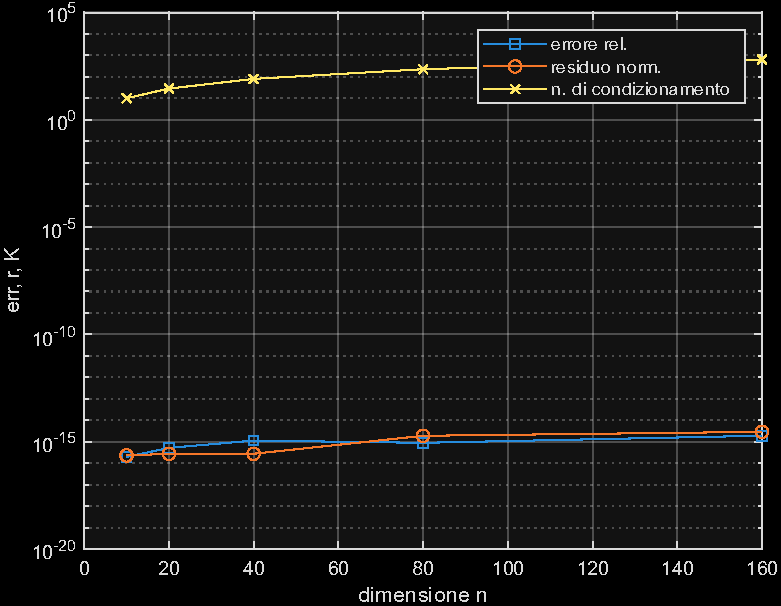
\includegraphics[width=.7\textwidth]{img/metodi-diretti.pdf}
        \caption{Andamento dell'errore relativo, del residuo normalizzato e del numero di condizionamento in funzione di $n$.}
    \end{figure}
\end{enumerate}

\newpage

\subsubsection{Metodi iterativi}

I metodi iterativi stazionari sono considerati in genere nella seguente forma:
\begin{equation*}
    \mathbf{x}^{\left(k+1\right)} = B\mathbf{x}^{\left(k\right)} + \mathbf{f} \hspace{2em} k \ge 0
\end{equation*}
Dove $B$ è detta matrice di iterazione. $B$ e $\mathbf{f}$ identificano il metodo.

\paragraph{Metodo di Jacobi}

Si consideri la matrice diagonale $D$ degli elementi diagonali di $A$. Tale matrice è facilmente invertibile, se gli $a_{ii} \ne 0, i = 1, \dots, n$, in quanto:
\begin{equation*}
    D = \begin{pmatrix}
        a_{11}  & 0     & 0     & \cdots    & 0     \\
        0       & a_{22}& 0     & \cdots    & 0     \\
        \vdots  & 0     & \ddots& \ddots    & \vdots\\
        \vdots  & \vdots& \ddots& \ddots    & 0     \\
        0       & 0     & \cdots& 0         & a_{nn}
    \end{pmatrix}
    \Longrightarrow
    D^{-1} = \begin{rowequmat}{ccccc}
        \dfrac{1}{a_{11}}   & 0                 & 0     & \cdots    & 0     \\ [.3em]
        0                   & \dfrac{1}{a_{22}} & 0     & \cdots    & 0     \\ [.3em]
        \vdots              & 0                 & \ddots& \ddots    & \vdots\\ [.3em]
        \vdots              & \vdots            & \ddots& \ddots    & 0     \\ [.3em]
        0                   & 0                 & \cdots& 0         & \dfrac{1}{a_{nn}}
    \end{rowequmat}
\end{equation*}
E il metodo può essere scritto direttamente in forma matriciale:
\begin{gather*}
    \mathbf{x}^{\left(0\right)} \text{ assegnato} \\
    \mathbf{x}^{\left(k+1\right)} = B_{J}\mathbf{x}^{\left(k\right)} + \mathbf{f}_{J} \\
\end{gather*}
Dove $B_{J} = I - D^{-1} A = D^{-1} \left(D-A\right)$ è la matrice di iterazione di Jacobi e $\mathbf{f}_{J} = D^{-1} \mathbf{b}$

\paragraph{Metodo di Gauss-Seidel}

Questo metodo si differenza dal metodo di Jacobi per il fatto che considera, oltre alla matrice $D$, anche le due matrici $-E$ e $-F$ triangolari superiore e inferiore della matrice $A$, ovvero:
\begin{equation*}
    -E = \begin{bmatrix}
        0 & 0 & 0 & \cdots &  0 \\
        a_{21} & 0 & 0 & \cdots & 0 \\
        \vdots & a_{32} & \ddots & \ddots & \vdots \\
        \vdots & \vdots & \ddots & \ddots & 0 \\
        a_{n1} & a_{n2} & \cdots & a_{nn-1} & 0
    \end{bmatrix}
    \hspace{2em}
    -F = \begin{bmatrix}
        0 & a_{12} & a_{13} & \cdots & a_{1n} \\
        0 & 0 & a_{23} & \cdots & a_{2n} \\
        \vdots & 0 & \ddots & \ddots & \vdots \\
        \vdots & \vdots & \ddots & \ddots & a_{n-1n} \\
        0 & 0 & \cdots & 0 & 0
    \end{bmatrix}
\end{equation*}
Dunque, il seguente algoritmo o le seguenti istruzioni:
\begin{gather*}
    \mathbf{x}^{\left(0\right)} \text{ assegnato} \\
    \mathbf{x}^{\left(k+1\right)} = B_{GS}\mathbf{x}^{\left(k\right)} + \mathbf{f}_{GS} \\
\end{gather*}
Dove $B_{GS} = \left(D-E\right)^{-1}F$ è la matrice d'iterazione di Gauss-Seidel e $\mathbf{f}_{GS} = \left(D-E\right)^{-1}\mathbf{b}$.

\paragraph{Esercizio}

Si considerino la matrice:
\begin{equation*}
    A = \begin{bmatrix}
        9 & -3 & 1 & & & & \\
        -3 & 9 & -3 & 1 & & & \\
        1 & -3 & 9 & -3 & 1 & & \\
        & 1 & -3 & 9 & -3 & 1 & \\
        && 1 & -3 & 9 & -3 & 1 \\
        &&& 1 & -3 & 9 & -3 \\
        &&&& 1 & -3 & 9 
    \end{bmatrix}
\end{equation*}
E il termine noto:
\begin{equation*}
    \mathbf{b} = \begin{bmatrix}
        7 & 4 & 5 & 5 & 5 & 4 & 7 
    \end{bmatrix}^{T}
\end{equation*}
\begin{enumerate}
    \item Costruire la matrice $A$ (utilizzando i comandi Matlab \texttt{diag} e \texttt{ones}) e determinare il numero di elementi non nulli tramite il comando \texttt{nnz}. La matrice $A$ è a dominanza diagonale per righe? È simmetrica e definita positiva?
    
    È stato richiesto di utilizzare i comandi \texttt{diag} e \texttt{ones} per costruire la matrice $A$. Quindi per farlo, si controlla rapidamente la documentazione dei due comandi:
    \begin{lstlisting}[language=bash]
>> help ones
 ones - Create array of all ones
    This MATLAB function returns the scalar 1.

    Syntax
      X = ones
      X = ones(n)
      X = ones(sz1,...,szN)
      X = ones(sz)

      X = ones(___,typename)
      X = ones(___,'like',p)

    Input Arguments
      n - Size of square matrix
        integer value
      sz1,...,szN - Size of each dimension
        two or more integer values
      sz - Output size
        row vector of integer values
      typename - Output class
        'double' (default) | 'single' | 'logical' | 'int8' | 'uint8' | ...
      p - Prototype
        variable

>> help diag
 diag - Create diagonal matrix or get diagonal elements of matrix
    This MATLAB function returns a square diagonal matrix with the elements
    of vector v on the main diagonal.

    Syntax
      D = diag(v)
      D = diag(v,k)

      x = diag(A)
      x = diag(A,k)

    Input Arguments
      v - Diagonal elements
        vector
      A - Input matrix
        matrix
      k - Diagonal number
        integer\end{lstlisting}
    Adesso si osservi la matrice $A$. È possibile notare che la diagonale principale ha tutti i valori uguale a $9$, mentre sopra e sotto la diagonale principale, altre due diagonali con valore pari a $-3$ e allo stesso modo due diagonali con valore uguale a $1$.

    Usando entrambi i comandi, si può giungere al seguente risultato parziale:
    \begin{lstlisting}[language=MATLAB]
>> diag(9*ones(1, n)) + diag(-3*ones(1,n-1), 1) + diag(1*ones(1,n-2), 2)

ans =

        9    -3     1     0     0     0     0
        0     9    -3     1     0     0     0
        0     0     9    -3     1     0     0
        0     0     0     9    -3     1     0
        0     0     0     0     9    -3     1
        0     0     0     0     0     9    -3
        0     0     0     0     0     0     9\end{lstlisting}
    Ed eseguendo con la stessa logica anche sotto la diagonale principale, si ottiene la matrice $A$ richiesta:
    \lstinputlisting[language=MATLAB]{code/risoluzione-di-sistemi-di-equazioni-lineari/metodi-iterativi/J_GS_1.m}

    Il numero di elementi non nulli si calcola con il comando \texttt{nnz}:
\begin{lstlisting}[language=bash]
>> help nnz
 nnz - Number of nonzero matrix elements
    This MATLAB function returns the number of nonzero elements in matrix X.

    Syntax
      N = nnz(X)

    Input Arguments
      X - Input matrix
        matrix

>> nnz(A)

ans =

    29
\end{lstlisting}
    E infine, per confermare che la matrice sia a dominanza diagonale per righe, simmetrica e definita positiva:
    \lstinputlisting[language=MATLAB]{code/risoluzione-di-sistemi-di-equazioni-lineari/metodi-iterativi/J_GS_2.m}


    \item Si calcolino le matrici di iterazione:
    \begin{gather*}
        B_{J} = D^{-1}\left(D - A\right) \\
        B_{GS} = \left(D - E\right)^{-1}F
    \end{gather*}
    Associate rispettivamente ai metodi di Jacobi e Gauss-Seidel e i relativi raggi spettrali. La condizione necessaria e sufficiente per la convergenza del metodo iterativo è soddisfatta in entrambi i casi?

    Le matrici di iterazione dei due metodi si calcolano a partire dalla definizione:
    \lstinputlisting[language=MATLAB]{code/risoluzione-di-sistemi-di-equazioni-lineari/metodi-iterativi/J_GS_3.m}

    Si noti l'istruzione \texttt{D = diag(diag(A))}; il comando interno estrae la diagonale principale di $A$, restituendo un vettore, il quale viene elaborato dal comando più esterno che crea una seconda matrice quadrata identica alla dimensione di $A$ ma con solo la diagonale principale.

    Dal calcolo del raggio spettrale delle matrici si può concludere che in questo caso entrambi i metodi convergono, in quanto l'autovalore massimo risulta in modulo strettamente minore di 1. Si osservi che il raggio spettrale della matrice di iterazione del metodo di Gauss-Seidel è più basso di quello della matrice del metodo di Jacobi.

    \item Scrivere la funzione Matlab che implementi il metodo di Jacobi inversione \emph{matriciale} per il sistema lineare $A\mathbf{x} = \mathbf{b}$. L'intestazione della funzione sarà la seguente:
    \begin{equation*}
        \texttt{[x,k] = jacobi(A,b,x0,toll,nmax).}
    \end{equation*}
    Il processo iterativo si arresta quando:
    \begin{equation*}
        \dfrac{\left|\left|\mathbf{r}^{(k)}\right|\right|}{\left|\left|\mathbf{b}\right|\right|} \leq \texttt{toll}
    \end{equation*}
    (criterio d'arresto del residuo normalizzato).

    \lstinputlisting[language=MATLAB]{code/risoluzione-di-sistemi-di-equazioni-lineari/metodi-iterativi/jacobi.m}

    \item Scrivere una funzione Matlab che implementi il metodo di Gauss-Seidel inversione \emph{matriciale} per il sistema lineare $A\mathbf{x} = \mathbf{b}$. L'intestazione della funzione sarà la seguente:
    \begin{equation*}
        \texttt{[x,k] = gs(A,b,x0,toll,nmax).}
    \end{equation*}

    \lstinputlisting[language=MATLAB]{code/risoluzione-di-sistemi-di-equazioni-lineari/metodi-iterativi/gs.m}

    \item Costruire il termine noto $\mathbf{b}$. Utilizzando le funzioni costruite nei punti 3 e 4, risolvere il sistema $A\mathbf{x} = \mathbf{b}$ ponendo $x^{(0)} = \left[0,0,\dots,0\right]^{T}$, $\texttt{toll} = 10^{-6}$ e $\texttt{nmax} = 1000$. Confrontare il numero di iterazioni necessarie per arrivare a convergenza per i due metodi e commentare i risultati ottenuti.
    
    Il metodo di Gauss-Seidel converge più velocemente alla soluzione esatta in accordo con il corrispondente raggio spettrale che è più basso di quello della matrice del metodo di Jacobi.
    \lstinputlisting[language=MATLAB]{code/risoluzione-di-sistemi-di-equazioni-lineari/metodi-iterativi/J_GS_4.m}
\end{enumerate}

\newpage

\paragraph{Metodo di Richardson}

Il metodo di Richardson stazionario è basato sulla seguente legge. Dati $\mathbf{x}^{\left(0\right)}$ e $\alpha \in \mathbb{R}$ si calcola:
\begin{equation}\label{lab-eq: metodo di Richardson}
    \mathbf{x}^{\left(k+1\right)} = \mathbf{x}^{\left(k\right)} + \alpha\mathbf{r}^{\left(k\right)} \hspace{2em} k \ge 0
\end{equation}
Dove $\alpha \ne 0$ è un parametro costante per ogni iterazione. Questo metodo richiede, ad ogni passo $k$, di calcolare il \emph{residuo} $\mathbf{r}^{\left(k\right)}$ definito come:
\begin{equation*}
    \mathbf{r}^{\left(k\right)} = \mathbf{b} - A \mathbf{x}^{\left(k\right)}
\end{equation*}
Il metodo di Richardson \emph{stazionario} converge solo per $0 < \alpha < \frac{2}{\lambda_{\max}}$, in cui $\lambda_{\max}$ è il massimo degli autovalori della matrice $A$. Inoltre, è possibile calcolare un valore di $\alpha$ ottimale che massimizza la velocità di convergenza. Questo valore è dato da:
\begin{equation*}
    \alpha_{\text{opt}} = \dfrac{2}{\lambda_{\min} + \lambda_{\max}}
\end{equation*}
In cui $\lambda_{\min}$ è il minimo degli autovalori della matrice $A$. Per questo valore, la velocità di convergenza è data da:
\begin{equation*}
    \rho_{\text{opt}} = \dfrac{K\left(A\right) - 1}{K\left(A\right) + 1}
\end{equation*}
Dove $K\left(A\right)$ è il numero di condizionamento, definito anche come:
\begin{equation*}
    K\left(A\right) = \left|\left| A^{-1} \right|\right| \cdot \left|\left| A \right|\right|
\end{equation*}
Dove $\left|\left| \cdot \right|\right|$ è una opportuna norma introdotta per la matrice. Vale sempre $K\left(A\right) \ge 1$. Se la matrice $A$ è simmetrica e definita positiva, utilizzando la sua norma 2, vale:
\begin{equation*}
    K\left(A\right) = \left|\left| A^{-1} \right|\right|_{2} \cdot \left|\left| A \right|\right|_{2} = \dfrac{\lambda_{\max}}{\lambda_{\min}}
\end{equation*}
Si noti che, dalla sua definizione, il metodo di Richardson (eq. \ref{lab-eq: metodo di Richardson}) può essere riscritto nella seguente forma (utilizzando la definizione di $\mathbf{r}$):
\begin{equation}
    \mathbf{x}^{\left(k+1\right)} = \left(I - \alpha A\right) \mathbf{x}^{\left(k\right)} + \alpha \mathbf{b} \hspace{2em} k \ge 0
\end{equation}
Segue che il metodo di Richardson è un metodo iterativo caratterizzato dalla matrice di iterazione $B_{\alpha} = I - \alpha A$ e da $\mathbf{f} = \alpha \mathbf{b}$.

\newpage

\paragraph{Precondizionamento}

Il numero di condizionamento di una matrice governa il rapporto tra l'errore relativo commesso dalla soluzione numerica nella risoluzione di un sistema lineare e il corrispondente residuo normalizzata, alla iterata $k$:
\begin{equation*}
    \dfrac{
        \left|\left| \mathbf{x}^{\left(k\right)} - \mathbf{x} \right|\right|
    }{
        \left|\left| \mathbf{x}^{\left(k\right)} \right|\right|
    } 
    \le
    K\left(A\right) \dfrac{
        \left|\left| \mathbf{r}^{\left(k\right)} \right|\right|
    }{
        \left|\left| \mathbf{b} \right|\right|
    }
\end{equation*}
Dove:
\begin{itemize}
    \item $\mathbf{x}^{\left(k\right)}$ è la soluzione numerica
    \item $\mathbf{r}^{\left(k\right)}$ è il residuo, ovvero $\mathbf{b} - A\mathbf{x}^{\left(k\right)}$
    \item $\mathbf{x}$ è la soluzione esatta del sistema lineare
\end{itemize}
Inoltre, nel caso del metodo di Richardson, si ottiene:
\begin{equation*}
    \left|\left| \mathbf{e}^{\left(k+1\right)} \right|\right|
    \le
    \dfrac{K\left(A\right)-1}{K\left(A\right)+1}
    \cdot
    \left|\left| \mathbf{e}^{\left(k\right)} \right|\right|
\end{equation*}
Come migliore stima ottenibile usando $\alpha_{\text{opt}}$.

\highspace
Per problemi ben condizionati ($K\left(A\right)$ non molto più grande di $1$), la soluzione del problema con piccoli residui non differisce molto dalla soluzione del problema originale; al contrario, in problemi con la matrice mal condizionata $\left(K\left(A\right) \gg  1\right)$ a piccoli residui possono corrispondere grandi errori e la convergenza è molto lenta.

\highspace
L'idea del precondizionamento consiste nel cercare di ridurre il numero di condizionamento della matrice del sistema, pre-moltiplicandola per una matrice $P^{-1}$ ($P$ è chiamata \emph{precondizionatore}). Si ottiene così il sistema equivalente:
\begin{equation*}
    P^{-1}A\mathbf{x}^{\left(k\right)} = P^{-1}\mathbf{b}
\end{equation*}
Ovviamente il precondizionatore è efficace se $K\left(P^{-1}A\right) \ll K\left(A\right)$ e se la soluzione del sistema lineare in $P$ che sorge ad ogni iterazione non è troppo onerosa. La prima proprietà è solitamente verificata quando $P^{-1} \approx A^{-1}$, cioè quando $P$ e $A$ hanno uno spettro simile, ma dovendo tener conto della seconda condizione è opportuno scegliere $P$ con una struttura speciale che mantenga basso il costo computazionale (ad esempio diagonale o triangolare).

\highspace
Ad esempio, nel caso di Richardson, per alleviare la dipendenza della convergenza ottimale dal numero di condizionamento, si introduce la tecnica di precondizionamento, che consiste nel sostituire $A$ con $P^{-1}A$. Questo metodo richiede, ad ogni iterata, di trovare il cosiddetto \emph{residuo precondizionato} $\mathbf{z}^{\left(k\right)}$ dato dalla soluzione del sistema lineare:
\begin{equation}\label{lab-eq: residuo precondizionato}
    P\mathbf{z}^{\left(k\right)} = \mathbf{r}^{\left(k\right)}
\end{equation}
Di conseguenza, la nuova iterata è definita da $\mathbf{x}^{\left(k+1\right)} = \mathbf{x}^{\left(k\right)} + \alpha\mathbf{z}^{\left(k\right)}$. Si noti che la matrice $P$, oltre ad essere non singolare (determinante diverso da zero), simmetrica (coincide con la sua trasposta) e definita positiva, deve essere scelta in modo tale che il costo computazionale richiesto dalla risoluzione del sistema (eq. \ref{lab-eq: residuo precondizionato}) sia basso. Per il caso precondizionato, valgono i precedenti risultati su $\alpha_{\text{opt}}$ e $\rho_{\text{opt}}$ a patto che si considerino gli autovalori di $P^{-1} A$ invece di quelli di $A$.

\longline

\paragraph{Metodo del gradiente}

È possibile generalizzare il metodo di Richardson precondizionato tramite l'introduzione di un parametro di accelerazione dinamico $\alpha_{k}$:
\begin{equation*}
    P\left(\mathbf{x}^{\left(k+1\right) - \mathbf{x}^{\left(k\right)}}\right) = \alpha_{k}\mathbf{r}^{\left(k\right)} \hspace{2em} k \ge 0, \: \alpha_{k} \ne 0
\end{equation*}
Con $P$ il precondizionatore. Lo scopo dell'utilizzo di $\alpha_{k}$ è quello di poter calcolare facilmente il parametro di accelerazione evitando il calcolo (spesso oneroso) degli autovalori di $A$ come per $\alpha_{\text{opt}}$. Questo metodo è detto \emph{metodo di Richardson dinamico}. Se $\alpha_{k}$ è scelto in modo ottimale, allora il metodo è detto del \emph{gradiente} se $P = I$, oppure del \emph{gradiente precondizionato} se $P \ne I$.

\highspace
A partire dal metodo di Richardson, è possibile ottenere i metodi del \emph{gradiente} ($P = I$) e del \emph{gradiente precondizionato} ($P \ne I$) tramite l'aggiunta del parametro $\alpha_{k}$: dato $\mathbf{x}^{\left(0\right)}$ assegnato, si ponga $\mathbf{r}^{\left(0\right)} = \mathbf{b} - A\mathbf{x}^{\left(0\right)}$ e per $k = 0, 1, \dots$
\begin{equation}
    \begin{array}{rcl}
        P\mathbf{z}^{\left(k\right)} &=& \mathbf{r}^{\left(k\right)} \\ [.5em]
        \alpha_{k} &=& \dfrac{
            \left(\mathbf{z}^{\left(k\right)}\right)^{T} \mathbf{r}^{\left(k\right)}
        }{
            \left(\mathbf{z}^{\left(k\right)}\right)^{T} A\mathbf{z}^{\left(k\right)}
        } \\ [2em]
        \mathbf{x}^{\left(k+1\right)} &=& \mathbf{x}^{\left(k\right)} + \alpha_{k} \mathbf{z}^{\left(k\right)} \\ [1em]
        \mathbf{r}^{\left(k+1\right)} &=& \mathbf{r}^{\left(k\right)} + \alpha_{k}A\mathbf{z}^{\left(k\right)}
    \end{array}
\end{equation}

\newpage

\paragraph{Esercizi su Richardson e gradiente}

Si considerino la matrice:
\begin{equation*}
    A = \begin{bmatrix}
        9 & -3 & 1 & & & & \\
        -3 & 9 & -3 & 1 & & & \\
        1 & -3 & 9 & -3 & 1 & & \\
        & 1 & -3 & 9 & -3 & 1 & \\
        && 1 & -3 & 9 & -3 & 1 \\
        &&& 1 & -3 & 9 & -3 \\
        &&&& 1 & -3 & 9 
    \end{bmatrix}
\end{equation*}
E il termine noto:
\begin{equation*}
    \mathbf{b} = \begin{bmatrix}
        7 & 4 & 5 & 5 & 5 & 4 & 7
    \end{bmatrix}^{T}
\end{equation*}
\begin{enumerate}
    \item Costruire la matrice $A$ (utilizzando i comandi Matlab \texttt{diag} e \texttt{ones}).
    \lstinputlisting[language=MATLAB]{code/risoluzione-di-sistemi-di-equazioni-lineari/metodi-iterativi/richardson_1.m}


    \item Calcolare l'intervallo di valori di $\alpha$ per cui il metodo di Richardson stazionario non precondizionato converge. Determinare il valore ottimale di $\alpha$ per avere massima velocità di convergenza.
    \lstinputlisting[language=MATLAB]{code/risoluzione-di-sistemi-di-equazioni-lineari/metodi-iterativi/richardson_2.m}


    \item Scrivere una funzione Matlab che implementi il metodo di Richardson stazionario non precondizionato per il sistema lineare $A\mathbf{x} = \mathbf{b}$. I parametri in ingresso richiesti dalla funzione sono la matrice $A$, il termine noto $\mathbf{b}$, il guess iniziale $\mathbf{x}^{\left(0\right)}$, il coefficiente $\alpha$, la tolleranza per il criterio d'arresto \texttt{toll} e il numero massimo di iterazioni ammesse \texttt{nmax}. La funzione restituisce la soluzione numerica $\mathbf{x}$ e il numero di iterazioni effettuate $k$.

    L'intestazione della funzione sarà la seguente:
    \begin{center}
        [x, k] = richardson(A, b, x0, alpha, toll, nmax)
    \end{center}
    Il processo iterativo si arresta quando:
    \begin{equation*}
        \dfrac{\left|\left| \mathbf{r}^{\left(k\right)} \right|\right|}{\left|\left| \mathbf{b} \right|\right|} \le \texttt{toll}
    \end{equation*}
    (criterio d'arresto del residuo normalizzato).
    \lstinputlisting[language=MATLAB]{code/risoluzione-di-sistemi-di-equazioni-lineari/metodi-iterativi/richardson.m}


    \item Costruire il termine noto $\mathbf{b}$. Utilizzando la funzione scritta al punto precedente, determinare la soluzione del sistema lineare $A\mathbf{x} = \mathbf{b}$, con $A$ data dal punto 1. 
    
    Si ponga $\mathbf{x}^{\left(0\right)} = \left[0, 0, \dots, 0\right]^{T}$, $\texttt{toll} = 10^{-6}$ e $\texttt{nmax} = 1000$. Si verifichi sperimentalmente che il metodo di Richardson stazionario non precondizionato converge solo se $\alpha$ appartiene all'intervallo trovato nel punto 2. In particolare, si scelga un $\alpha$ al di fuori dell'intervallo e si verifichi che il metodo diverge. Si provi, inoltre, sperimentalmente, che per $\alpha_{\text{opt}}$ il metodo converge più velocemente. In particolare, si scelga un $\alpha$ nell'intervallo di convergenza e si osservi il numero di iterazioni per aggiungere a convergenza è maggiore di quello ottenuto utilizzando $\alpha_{\text{opt}}$.
    \lstinputlisting[language=MATLAB]{code/risoluzione-di-sistemi-di-equazioni-lineari/metodi-iterativi/richardson_3.m}
\end{enumerate}

\longline

\noindent
Adesso si passa al gradiente. Si consideri il problema lineare $A\mathbf{x} = \mathbf{b}$, dove la matrice $A \in \mathbb{R}^{n \times n}$ è pentadiagonale:
\begin{equation*}
    A = \begin{bmatrix}
        4 & -1 & -1 & & & & \\
        -1 & 4 & -1 & -1 & & & \\
        -1 & 4 & -1 & -1 & -1 & & \\
         & \ddots & \ddots & \ddots & \ddots & \ddots & \\
         & & -1 & -1 & 4 & -1 & -1 \\
         & & & -1 & -1 & 4 & -1 \\
         & & & & -1 & -1 & 4 \\
    \end{bmatrix}
    \hspace{1em}
    \mathbf{b} = \begin{bmatrix}
        0.2 \\ 0.2 \\ 0.2 \\ \vdots \\ 0.2 \\ 0.2 \\ 0.2
    \end{bmatrix}
\end{equation*}
Si vuole risolvere tale problema con il metodo del gradiente, soddisfando una tolleranza di $10^{-5}$ per il criterio relativo al residuo normalizzato, a partire dal vettore iniziale $\mathbf{x}_{0} = \left[0, \dots, 0\right]^{T}$.
\begin{enumerate}
    \item Costruire la matrice $A$ con $n = 50$, il termine noto $\mathbf{b}$ ed il vettore soluzione iniziale $\mathbf{x}_{0}$. La matrice $A$ è simmetrica e definita positiva? Se ne calcoli il numero di condizionamento, senza utilizzare il comando \texttt{cond} di Matlab.
    \lstinputlisting[language=MATLAB]{code/risoluzione-di-sistemi-di-equazioni-lineari/metodi-iterativi/gradiente_1.m}
    \newpage
    \begin{figure}[!htp]
        \centering
        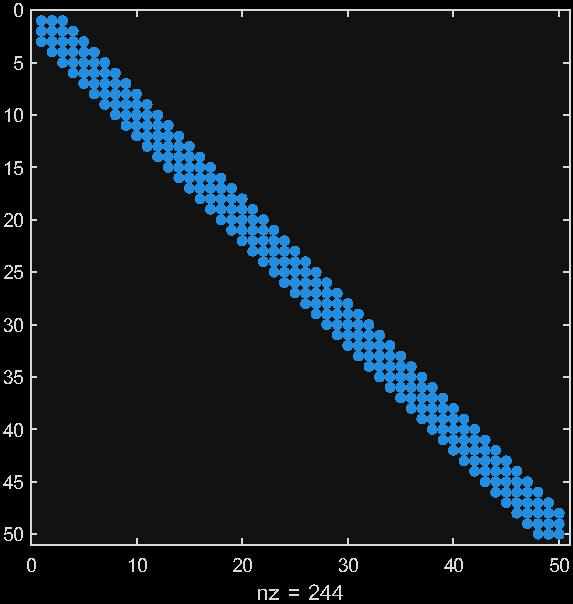
\includegraphics[width=.6\textwidth]{img/gradiente-1.pdf}
    \end{figure}

    \item Si scriva una funzione che implementi il metodo del gradiente e la si usi per risolvere il sistema lineare $A\mathbf{x} = \mathbf{b}$. L'intestazione della funzione sarà ad esempio:
    \begin{center}
        \texttt{[x, iter, err] = graddyn(A, b, x0, nmax, toll)}
    \end{center}
    Dove \texttt{err} è il vettore contenente il residuo normalizzato ad ogni iterazione.
    \lstinputlisting[language=MATLAB]{code/risoluzione-di-sistemi-di-equazioni-lineari/metodi-iterativi/graddyn.m}

    \item Utilizzare la funzione scritta al punto precedente per determinare la soluzione del sistema lineare $A\mathbf{x} = \mathbf{b}$.
    \lstinputlisting[language=MATLAB]{code/risoluzione-di-sistemi-di-equazioni-lineari/metodi-iterativi/gradiente_2.m}

    \item A partire dal \texttt{graddyn.m}, si scriva una funzione \texttt{gradprec.m} che implementi il metodo del gradiente precondizionato. L'intestazione della funzione sarà ad esempio:
    \begin{center}
        \texttt{[x, iter, err] = gradprec(A, b, x0, nmax, toll)}
    \end{center}
    Si risolva il sistema lineare $A\mathbf{x} = \mathbf{b}$ applicando il metodo del gradiente precondizionato con il precondizionatore:
    \begin{equation*}
        P = \begin{bmatrix}
            2 & -1 & & & \\
            -1 & 2 & -1 & & \\
             & \ddots & \ddots & \ddots & \\
             & & -1 & 2 & -1 \\
             & & & -1 & 2 \\
        \end{bmatrix}
    \end{equation*}
    \lstinputlisting[language=MATLAB]{code/risoluzione-di-sistemi-di-equazioni-lineari/metodi-iterativi/gradprec.m}
    \lstinputlisting[language=MATLAB]{code/risoluzione-di-sistemi-di-equazioni-lineari/metodi-iterativi/gradiente_3.m}

    \item Disegnare su un grafico l'andamento del residuo normalizzato:
    \begin{equation*}
        \dfrac{\left|\left| \mathbf{r}^{\left(k\right)} \right|\right|}{\left|\left| \mathbf{b} \right|\right|}
    \end{equation*}
    In funzione delle iterazioni $k$ nei due casi (gradiente e gradiente precondizionato), e confrontare le curve ottenute.
    \lstinputlisting[language=MATLAB]{code/risoluzione-di-sistemi-di-equazioni-lineari/metodi-iterativi/gradiente_4.m}
    \begin{figure}[!htp]
        \centering
        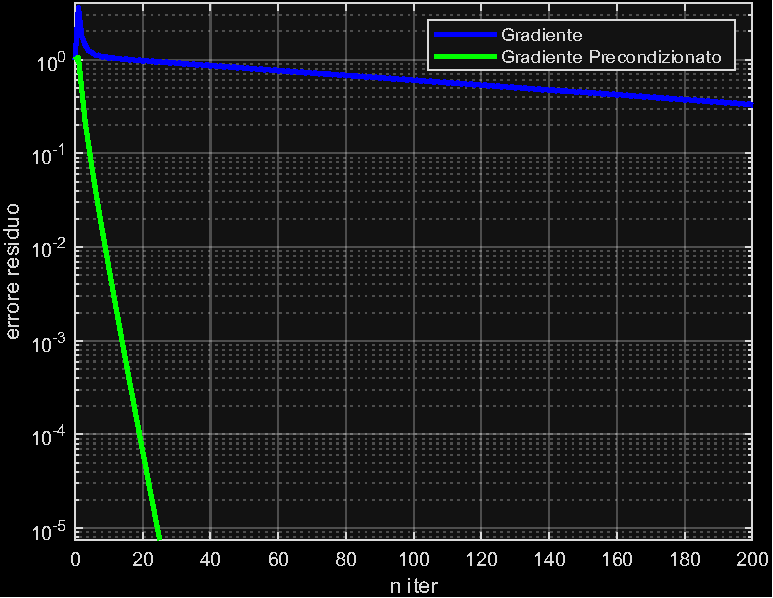
\includegraphics[width=.7\textwidth]{img/gradiente-2.pdf}
    \end{figure}

    \item A partire da \texttt{richardson.m}, si scriva una funzione \texttt{richprec.m} che implementi il metodo di Richardson precondizionato. L'intestazione della funzione sarà ad esempio:
    \begin{center}
        \texttt{[x, iter, err] = richprec(A, b, P, alpha, x0, nmax, toll)}
    \end{center}
    Si risolva il sistema lineare $A\mathbf{x} = \mathbf{b}$ applicando il metodo di Richardson precondizionato utilizzando la relativa $\alpha_{\text{opt}}$ e il precondizionatore $P$ implementato al punto 4.
    \lstinputlisting[language=MATLAB]{code/risoluzione-di-sistemi-di-equazioni-lineari/metodi-iterativi/richprec.m}
    \lstinputlisting[language=MATLAB]{code/risoluzione-di-sistemi-di-equazioni-lineari/metodi-iterativi/gradiente_5.m}

    \item Si risolva il sistema lineare $A\mathbf{x} = \mathbf{b}$ con il metodo di Richardson. Disegnare su un grafico l'andamento del residuo normalizzato:
    \begin{equation*}
        \dfrac{\left|\left| \mathbf{r}^{\left(k\right)} \right|\right|}{\left|\left| \mathbf{b} \right|\right|}
    \end{equation*}
    In funzione delle iterazioni $k$ nei due casi (Richardson e Richardson precondizionato), e confrontare le curve ottenute.
    \lstinputlisting[language=MATLAB]{code/risoluzione-di-sistemi-di-equazioni-lineari/metodi-iterativi/gradiente_6.m}
    \newpage
    \begin{figure}[!htp]
        \centering
        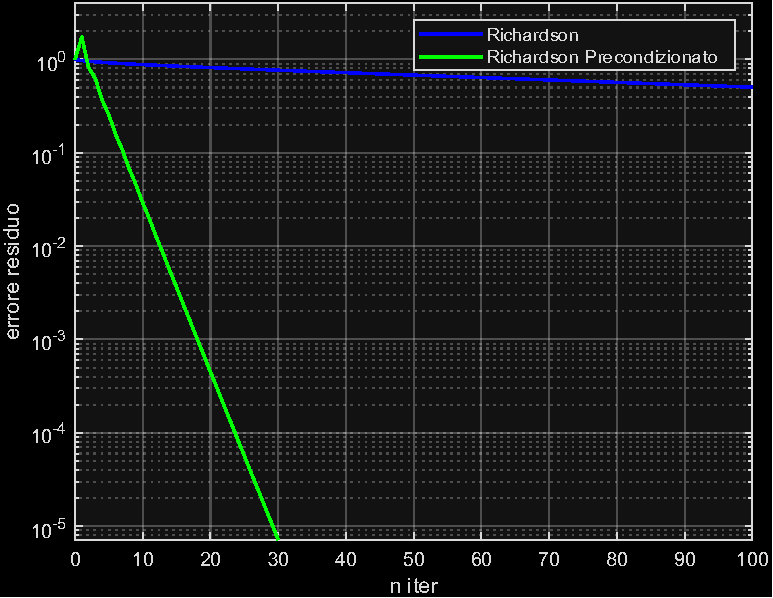
\includegraphics[width=.7\textwidth]{img/gradiente-3.pdf}
    \end{figure}
\end{enumerate}